\Opensolutionfile{ans}[ans/ansCD2D1-2-1]
\setcounter{section}{1}
\section{CỰC TRỊ CỦA HÀM SỐ}
\subsection{Lý thuyết cần nắm}
\subsubsection{Khái niệm cực đại, cực tiểu}
\begin{center}
	\begin{tikzpicture}[scale=1, font=\footnotesize, line join=round, line cap=round,>=stealth]
	\draw[->] (-6,0)--(6,0) node[below]{$x$};
	\draw[->] (0,-1.5)--(0,4.5) node[right]{$y$};
	\coordinate[label=below left:$O$] (O) at (0,0);	
	\coordinate (A) at (-6,4);
	\coordinate (B) at (-4,2);
	\coordinate (C) at (-3,3);
	\coordinate (D) at (-1,-1);
	\coordinate (E) at (3,3.5);
	\coordinate (F) at (5,1.2);	
	\draw 
	(A) .. controls +(-50:0.4) and +(-170:0.1) ..
	(B) .. controls +(80:0.3) and +(170:0.4) ..
	(C) .. controls +(0:0.6) and +(180:.5) ..
	(D) .. controls +(0:1) and +(-175:.6) ..
	(E) .. controls +(-60:0.5) and +(160:1) ..(F);
	
	\draw[dashed] (-4,0)node[below left]{Điểm}--(B) (-3.5,0)node[below]{$a$}--(-3.5,2.8);
	\node at (-4,-0.7)[left]{cực tiểu};
	\draw[dashed] (-3,0)node[below]{Điểm}--(C) (-2.5,0)node[above right]{$b$}--(-2.5,2.5);
	\node at (-3,-0.7){cực đại};
	\node at (-1,0.7){Điểm};
	\draw[dashed] (-1,0)node[above]{cực tiểu}--(D);
	\draw[dashed] (3,0)node[below]{Điểm}--(E);
	\node at (3,-0.7){cực đại};
	\draw (-3.5,3)--(-2.5,3) (-1.5,-1)--(-0.5,-1) (2.5,3.5)--(3.5,3.5);
	\fill (0,0) circle (1.0pt) (-1,0) circle (1.0pt) (-4,0) circle (1.0pt) (-3,0) circle (1.0pt) (-3.5,0) circle (1.0pt) (3,0) circle (1pt) (-2.5,0) circle (1pt);
	\end{tikzpicture}
\end{center}
Cho hàm số $y=f(x)$ xác định, liên tục trên $\mathscr{D}, x_0\in \mathscr{D}$.
\begin{dn}
\begin{itemize}
	\item Nếu tồn tại khoảng $(a;b)\subset \mathscr{D},x_0\in (a;b)$ sao cho $f(x)<f(x_0)$ với mọi $x\in (a; b)$ và $x\neq x_0$ thì ta nói hàm số $f(x)$ đạt cực đại tại điểm $x_0$.
	\item Nếu tồn tại khoảng $(a;b)\subset \mathscr{D},x_0\in (a;b)$ sao cho $f(x)>f(x_0)$ với mọi $x\in (a; b)$ và $x\neq x_0$ thì ta nói hàm số $f(x)$ đạt cực đại tại điểm $x_0$.
\end{itemize}
\end{dn}
\begin{note}
\begin{itemize}
	\item Nếu hàm số $y=f(x)$ đạt cực đại (cực tiểu) tại $x_0$ thì
		\begin{itemize}
			\item $x_0$ được gọi là \textbf{điểm cực đại (điểm cực tiểu)} của hàm số,
			\item $f(x_0)$ được gọi là \textbf{giá trị cực đại (hoặc giá trị cực tiểu)} của hàm số, kí hiệu $y_{\text{CĐ}}$, $y_{\text{CT}}$;
			\item điểm $M(x_0;f(x_0))$ gọi là \textbf{điểm cực đại (hoặc điểm cực tiểu)} của đồ thị hàm số.
		\end{itemize}
	\item Các điểm cực đại và cực tiểu gọi chung là điểm cực trị. Giá trị cực đại (giá trị cực tiểu) còn gọi là cực đại (cực tiểu) và được gọi chung là cực trị của hàm số.
	\item Giá trị cực đại (cực tiểu) $f(x_0)$ của hàm số $y=f(x)$ nói chung không phải là giá trị lớn nhất (nhỏ nhất) của hàm số trên tập xác định $\mathscr{D}, f(x_0)$ chỉ là giá trị lớn nhất (nhỏ nhất) của hàm số $y=f(x)$ trên một khoảng $(a;b)\subset \mathscr{D}$ nào đó chứa (lân cận) điểm $x_0$. (sẽ nhắc lại kĩ hơn ở bài sau "GTLN, GTNN của hàm số")
\end{itemize}
\end{note}
\subsubsection{Các định lí.}
\begin{dl}[điều kiện cần]
	Nếu hàm số $y=f(x)$ có đạo hàm trên khoảng $(a;b)$ và đạt cực đại (hoặc cực tiểu) tại $x_0$ thì $f'(x_0)=0$.
\end{dl}
\begin{dl}[điều kiện đủ]
\quad
\begin{center}
	\begin{tikzpicture}
	\tkzTabInit[nocadre=false,lgt=1.2,espcl=1.5]
	{$x$ /0.6,$f'(x)$/0.6,$f(x)$ /2}
	{$-\infty$,$x_0$,$+\infty$}
	\tkzTabLine{,+,|,-,}
	\tkzTabVar{-/, +/$y_{\text{CĐ}}$,-/}
	\end{tikzpicture}
	\quad
	\begin{tikzpicture}
	\tkzTabInit[nocadre=false,lgt=1.2,espcl=1.5]
	{$x$ /0.6,$f'(x)$/0.6,$f(x)$ /2}
	{$-\infty$,$x_0$,$+\infty$}
	\tkzTabLine{,-,|,+,}
	\tkzTabVar{+/, -/$y_{\text{CT}}$,+/}
	\end{tikzpicture}
\end{center}
• Nếu $f'(x)$ đổi dấu từ \textbf{dương sang âm} khi $x$ đi qua điểm $x_0$ (theo chiều tăng) thì hàm số $y=f(x)$ đạt \textbf{cực đại} tại điểm $x_0$.\\
• Nếu $f'(x)$ đổi dấu từ \textbf{âm sang dương} khi $x$ đi qua điểm $x_0$ (theo chiều tăng) thì hàm số $y=f(x)$ đạt \textbf{cực tiểu} tại điểm $x_0$.
\end{dl}
\begin{dl}
Giả sử $y=f(x)$ có đạo hàm cấp $2$ trong khoảng $(a; b)$. Khi đó:
\begin{itemize}
	\item Nếu $y'(x_0)=0, y''(x_0)>0$ thì $x_0$ là điểm cực tiểu.
	\item Nếu $y'(x_0)=0, y''(x_0)<0$ thì $x_0$ là điểm cực đại.
	\item Nếu $y'(x_0)=0, y''(x_0)=0$ thì chưa có kết luận về cực trị của hàm số.
\end{itemize}
\end{dl}
\begin{note}
Một hàm số chỉ có thể đạt cực trị tại một điểm mà tại đó đạo hàm của hàm số bằng $0$, hoặc tại đó hàm số không có đạo hàm, chẳng hạn hàm số $y=|x|$.
\end{note}
\subsection{Phân loại và phương pháp giải bài tập}
\begin{dang}{Tìm cực trị của hàm số}
Bài toán: Tìm các điểm cực đại, cực tiểu (nếu có) của hàm số $y=f(x)$
	Phương pháp: Sử dụng hai cách tìm cực trị sau:\\
	\textbf{Cách 1:} \textit{(Sử dụng nội dung định lý 2)} Lập bảng biến thiên. Từ bảng biến thiên, suy ra các điểm cực trị (dựa vào nội dung định lý 2).\\
	\textbf{Cách 2.} \textit{(Sử dụng nội dung định lý 3)}\\ 
	\textbf{Bước 1.} Tìm tập xác định $\mathscr{D}$ của hàm số.\\
	\textbf{Bước 2.} Tính đạo hàm $y'=f'(x)$. Giải $f'(x)=0$ và kí hiệu $x_i, (i=1, 2, 3,\ldots,n)$ là các nghiệm của nó.\\
	\textbf{Bước 3.} Tính $f''(x)$ và $f''(x_i)$.\\
	\textbf{Bước 4.} Dựa vào dấu của $f''(x_i)$ suy ra tính chất cực trị của điểm $x_i\colon$.\\
	+ Nếu $f''(x_i)<0$ thì hàm số đạt cực đại tại điểm $x_i$.\\
	+ Nếu $f''(x_i)>0$ thì hàm số đạt cực tiểu tại điểm $x_i$.
\end{dang}
\paragraph{Các ví dụ}
\begin{vd}%Câu 1.%[2D1B2-1]
	Tìm điểm cực trị của hàm số $y=x^3-3x^2-24x+7$.
\end{vd}
\begin{vd}%Câu 2.%[2D1B2-1]
	Tìm cực trị của hàm số $y=x^4-2x^2+3$.
\end{vd}
\begin{vd}%Câu 3.%[2D1B2-1]
	Tìm cực trị của hàm số $y=-x^3+3x^2-3x+1$.
\end{vd}
\begin{vd}%Câu 4.%[2D1B2-1]
	Tìm cực trị của hàm số $y=\dfrac{2x+1}{x-3}$.
\end{vd}
\begin{vd}%Câu 5.%[2D1B2-1]
	Tìm cực trị của hàm số $y=\dfrac{2x^2+x+1}{x+1}$.
\end{vd}
\begin{vd}%Câu 6.%[2D1B2-1]
	Tìm cực trị của hàm số $y=\sqrt{5-4x-x^2}$.
\end{vd}
\begin{vd}%Câu 7.%[2D1Y2-1]
	Tìm giá trị cực tiểu $y_{\text{CT}}$ của hàm số $y=x^3+3x^2-3$. 
	\choice
	{$y_{\text{CT}}=0$}
	{\True $y_{\text{CT}}=-3$}
	{$y_{\text{CT}}=9$}
	{$y_{\text{CT}}=1$}
	\loigiai{
		Ta có $y'=3x^2+6x,y'=0\Leftrightarrow\hoac{&x=0\\&x=-2.}$ \\
		Bảng biến thiên: 
		\begin{center}
			\begin{tikzpicture}
			\tkzTabInit[nocadre=false,lgt=1.2,espcl=2.5,deltacl=0.6]
			{$x$ /0.6, $y'$ /0.6, $y$ /2.5}
			{$-\infty$,$-2$,$0$,$+\infty$}
			\tkzTabLine{,+,$0$,-,$0$,+,}
			\tkzTabVar{-/$-\infty$,+/$1$,-/$-3$,+/$+\infty$}
			\end{tikzpicture}
	\end{center}}
\end{vd}
\begin{vd}%Câu 12.%[2D1B2-1]
	Cho hàm số $y=x^4-8x^2+10$ có đồ thị $(C)$. Gọi $A$, $B$, $C$ là $3$ điểm cực trị của đồ thị $(C)$. Tính diện tích $S$ của tam giác $ABC$. 
	% \choice
	% {$S=64$}
	% {\True $S=32$}
	% {$S=24$}
	% {$S=12$}
	\loigiai{
		Ta có $y'=4x^3-16x$; $y'=0\Leftrightarrow\hoac{&x=0\Rightarrow y=10\\&x=2\Rightarrow y=-6\\&x=-2\Rightarrow y=-6.}$ \\
		Không mất tính tổng quát giả sử $A(0;10)$, $B(2;-6)$, $C(-2;-6)$
		Tam giác $ABC$ cân tại $A$. Gọi $H$ là trung điểm của $BC$, khi đó $H(0;-6)$
		Diện tích tam giác $ABC$ là $S=\dfrac{1}{2}AH\cdot BC=\dfrac{1}{2}\cdot 16\cdot 4=32$.}
\end{vd}
\begin{vd}%Câu 13.%[2D1K2-2]
	\immini{
		Cho hàm số $y=f(x)$ có đạo hàm $f'(x)$ trên khoảng $(-\infty;+\infty)$. Đồ thị của hàm số $y=f(x)$ như hình vẽ. Đồ thị của hàm số $y=\left(f(x)\right)^2$ có bao nhiêu điểm cực đại, cực tiểu?
	% \choice
	% {\True $2$ điểm cực đại, $3$ điểm cực tiểu}
	% {$1$ điểm cực đại, $3$ điểm cực tiểu}
	% {$2$ điểm cực đại, $2$ điểm cực tiểu}
	% {$3$ điểm cực đại, $2$ điểm cực tiểu}
	}{
		\begin{tikzpicture}[scale=0.7, font=\footnotesize, line join=round, line cap=round,>=stealth]
		\def\a{1}  % Hệ số co dãn
		\def\xmin{-1} \def\xmax{4}
		\def\ymin{-3.1} \def\ymax{3} 
		\draw[->] (\xmin,0)--(\xmax,0) node [below]{$x$};
		\draw[->] (0,\ymin)--(0,\ymax) node [right]{$y$};
		\node at (0,0) [below left]{$O$};
		\clip (\xmin+0.1,\ymin+0.1) rectangle (\xmax-0.1,\ymax-0.1);
		\draw[smooth,samples=300,domain=-0.5:3.5] plot(\x,{\a*((\x-1)^2*(\x)*(\x-3))});
		\fill (0,0) circle (1.0pt) (1,0) circle (1.0pt)node[above]{$1$} (3,0) circle (1.0pt)node[above left]{$3$};
		\end{tikzpicture}
	}
	\loigiai{
		Từ đồ thị hàm số ta có bảng biến thiên
		\begin{center}
			\begin{tikzpicture}
			\tkzTabInit[nocadre=false,lgt=1.2,espcl=2.5,deltacl=0.6]
			{$x$ /0.6,$f'(x)$ /0.6,$f(x)$ /2}
			{$-\infty$,$x_1$,$1$,$x_2$,$+\infty$}
			\tkzTabLine{,-,$0$,+,$0$,-,$0$,+,}
			\tkzTabVar{+/$+\infty$, -/$y_1$,+/$0$,-/$y_2$,+/$+\infty$}
			\end{tikzpicture}
		\end{center}
		$y=\left(f(x)\right)^2\Rightarrow y'=2f(x)\cdot f'(x)=0\Leftrightarrow\hoac{&f(x)=0\\&f'(x)=0.}$ \\
		Quan sát đồ thị ta có $f(x)=0\Leftrightarrow\hoac{&x=0\\&x=1\\&x=3}$ và $f'(x)=0\Leftrightarrow\hoac{&x=x_1\\&x=1\\&x=x_2}$ với $x_1\in(0;1)$ và $x_2\in(1;3)$.\\
		Suy ra $y'>0\Leftrightarrow\hoac{&\heva{&f(x)>0\\&f'(x)>0}\\&\heva{&f(x)<0\\&f'(x)<0}}\Leftrightarrow\hoac{&x\in(3;+\infty)\\&x\in(0;x_1)\cup(1;x_2)}\Leftrightarrow x\in(0;x_1)\cup(1;x_2)\cup(3;+\infty)$.\\
		Từ đó ta lập được bảng biến thiên của hàm số $y=\left(f(x)\right)^2$ 
		\begin{center}
			\begin{tikzpicture}
			\tkzTabInit[nocadre=false,lgt=1,espcl=2.3,deltacl=0.6]
			{$x$ /0.6,$y'$ /0.6,$y$ /2}
			{$-\infty$,$0$,$x_1$,$1$,$x_2$,$3$,$+\infty$}
			\tkzTabLine{,-,$0$,+,$0$,-,$0$,+,$0$,-,$0$,+,}
			\tkzTabVar{+/$+\infty$,-/,+/$y_1$,-/,+/$y_2$,-/,+/$+\infty$}
			\end{tikzpicture}
		\end{center}
		Suy ra hàm số có $2$ điểm cực đại, $3$ điểm cực tiểu.}
\end{vd}
\paragraph{Câu hỏi trắc nghiệm}
\begin{ex}%Câu 8.%[2D1Y2-2]
	Cho hàm số $y=f(x)$ có bảng biến thiên như sau: 
	\begin{center}
		\begin{tikzpicture}
		\tkzTabInit[nocadre=false,lgt=1.2,espcl=2.5,deltacl=0.6]
		{$x$ /0.6, $y'$ /0.6, $y$ /2.5}
		{$-\infty$,$0$,$3$,$+\infty$}
		\tkzTabLine{,+,$0$,-,$0$,+,}
		\tkzTabVar{-/$-\infty$,+/$2$,-/$-2$,+/$+\infty$}
		\end{tikzpicture}
	\end{center}
	Tìm giá trị cực đại và giá trị cực tiểu của hàm số đã cho. 
	\choice
	{$y_{\text{CĐ}}=3$ và $y_{\text{CT}}=0$}
	{\True $y_{\text{CĐ}}=2$ và $y_{\text{CT}}=-2$}
	{$y_{\text{CĐ}}=-2$ và $y_{\text{CT}}=2$}
	{$y_{\text{CĐ}}=0$ và $y_{\text{CT}}=3$.}
\end{ex}
\begin{ex}%Câu 9.%[2D1Y2-2]
	\immini{
		Cho hàm số $y=f(x)$ liên tục trên $\mathbb{R}$ và có đồ thị là đường cong như hình vẽ bên. Tìm điểm cực tiểu của đồ thị hàm số $y=f(x)$. 	
	\choice
	{$y=-2$}
	{\True $M(0;-2)$}
	{$x=0$}
	{$N(2;2)$}
	}{
		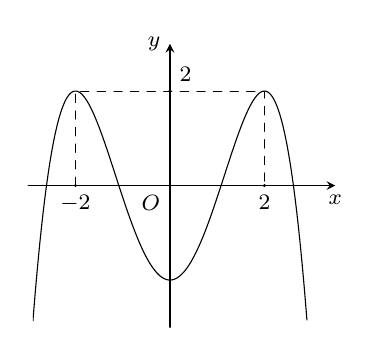
\begin{tikzpicture}[scale=0.6, font=\footnotesize, line join=round, line cap=round,>=stealth]
		\def\a{-1} \def\b{8} \def\c{-2} % Hệ số
		\def\xmin{-3} \def\xmax{3.5}
		\def\ymin{-3} \def\ymax{3} 
		\draw[->] (\xmin,0)--(\xmax,0) node [below]{$x$};
		\draw[->] (0,\ymin)--(0,\ymax) node [left]{$y$};
		\node at (0,0) [below left]{$O$};
		\clip (\xmin+0.1,\ymin+0.1) rectangle (\xmax-0.1,\ymax-0.1);
		\draw[smooth,samples=300,domain=-2.9:2.9] plot(\x,{1/4*(\a*(\x)^4+\b*(\x)^2)+\c});
		\draw[dashed] (-2,0)node[below]{$-2$}--(-2,2)--(2,2)--(2,0)node[below]{$2$};
		\fill (0,0) circle (1.0pt) (0,2) circle (1.0pt)node[above right]{$2$} (2,0) circle (1.0pt) (-2,0) circle (1.0pt);
		\end{tikzpicture}
	}
	\loigiai{
		Từ đồ thị ta có đồ thị hàm số đạt cực tiểu tại $M(0;-2)$.}
\end{ex}
\begin{ex}%Câu 1.%[2D1B2-1]
	Điểm cực tiểu của đồ thị hàm số $y=x^3-3x+5$ là điểm?
	\choice
	{$Q(3; 1)$}
	{\True $M(1; 3)$}
	{$P(7;-1)$}
	{$N(-1; 7)$}
	\loigiai{
		Ta có $y'=3x^2-3\Rightarrow y''=6x$
		Khi đó $y'=0\Leftrightarrow\hoac{&x=1\Rightarrow y''(1)=6>0\\&x=-1\Rightarrow y''(-1)=-6<0}$ \\
		$ \Rightarrow $ Hàm số đạt cực tiểu tại $x=1$ và hàm số đạt cực đại tại $x=-1$
		Với $x=1\Rightarrow y=3\Rightarrow$ điểm cực tiểu của đồ thị hàm số $y=x^3-3x+5$ là $M(1; 3)$.}
\end{ex}
\begin{ex}%Câu 2.%[2D1B2-1]
	Tìm điểm cực đại của đồ thị hàm số $y=x^4-2x^2+2$. 
	\choice
	{$(-1;1)$}
	{$(2;0)$}
	{$(1;1)$}
	{\True $(0;2)$}
	\loigiai{
		Ta có $y'=4x^3-4x$. $y'=0\Leftrightarrow\hoac{&x=1\\&x=-1\\&x=0.}$ \\
		$y''=12x^2-4$
		$y''(0)=-4\Rightarrow$ điểm cực đại.\\
		$y''(1)=8$.\\
		$y''(-1)=8$.}
\end{ex}
\begin{ex}%Câu 3.%[2D1Y2-1]
	Cho hàm số $y=f(x)$ có $f'(x)=(2x-1)x^2(1-x)^2$. Khẳng định nào sau đây là khẳng định đúng?
	\choice
	{Hàm số đã cho không có cực trị}
	{\True Hàm số đã cho có đúng một cực trị}
	{Hàm số đã cho có hai cực trị}
	{Hàm số đã cho có ba cực trị}
	\loigiai{
		$f'(x)$ chỉ đổi dấu qua nghiệm $x=\dfrac{1}{2}$ nên hàm số đã cho có đúng một cực trị.}
\end{ex}
\begin{ex}%Câu 4.%[2D1Y2-1]
	Hàm số $y=\dfrac{2x+1}{x-1}$ có bao nhiêu điểm cực trị?
	\choice
	{\True $0$}
	{$2$}
	{$1$}
	{$3$}
	\loigiai{
		Ta có $y'=-\dfrac{3}{(x-1)^2}<0;\forall x\neq 1$ nên hàm số không có cực trị.}
\end{ex}
\begin{ex}%Câu 5.%[2D1Y2-1]
	Số điểm cực trị của hàm số $y=x^5+2x^4+2018$ là 
	\choice
	{$3$}
	{$0$}
	{$4$}
	{\True $2$}
	\loigiai{
		Tập xác định: $\mathscr{D}=\mathbb{R}$, $y'=5x^4+8x^3$, $y'=0\Leftrightarrow 5x^4+8x^3=0\Leftrightarrow\hoac{&x=0\\&x=-\dfrac{8}{5}.}$ \\
		Ta có bảng biến thiên của hàm số: 
		\begin{center}
			\begin{tikzpicture}
			\tkzTabInit[nocadre=false,lgt=1.2,espcl=2.5,deltacl=0.6]
			{$x$ /1, $y'$ /1, $y$ /2.5}
			{$-\infty$,$-\dfrac{8}{5}$,$0$,$+\infty$}
			\tkzTabLine{,+,$0$,-,$0$,+,}
			\tkzTabVar{-/,+/,-/,+/}
			\end{tikzpicture}
		\end{center}
		Vậy hàm số có $2$ cực trị.}
\end{ex}
\begin{ex}%Câu 6.%[2D1B2-1]
	Điểm cực tiểu của hàm số $y=x\sqrt{4-x^2}$ là
	\choice
	{$x=-2\sqrt{3}$}
	{$x=2$}
	{\True $x=-\sqrt{2}$}
	{$x=\sqrt{2}$}
	\loigiai{
		Tập xác định $\mathscr{D}=[-2;2]$.\\
		$y'=\sqrt{4-x^2}-\dfrac{x^2}{\sqrt{4-x^2}}=\dfrac{4-2x^2}{\sqrt{4-x^2}}$.\\
		$y'=0\Leftrightarrow x=\pm\sqrt{2}$.\\
		Bảng biến thiên
		\begin{center}
			\begin{tikzpicture}
			\tkzTabInit[nocadre=false,lgt=1.2,espcl=2.2,deltacl=0.6]
			{$x$ /0.6, $y'$ /0.6, $y$ /2.5}
			{$-2$,$-\sqrt{2}$,$\sqrt{2}$,$2$}
			\tkzTabLine{,-,$0$,+,$0$,-,}
			\tkzTabVar{+/,-/,+/,-/}
			\end{tikzpicture}
		\end{center}
		Dựa vào bảng biến thiên suy ra điểm cực tiểu của hàm số là $x=-\sqrt{2}$.}
\end{ex}
\begin{ex}%Câu 10.%[2D1Y2-1]
	Cho hàm số $y=x^5-2x^4+x^3-1$. Số điểm cực trị của hàm số là
	\choice
	{\True $2$}
	{$0$}
	{$1$}
	{$4$}
	\loigiai{
		$y=x^5-2x^4+x^3-1\Rightarrow y'=5x^4-8x^3+3x^2$
		$y'=0\Leftrightarrow 5x^4-8x^3+3x^2=0\Leftrightarrow\hoac{&x=0\\&x=1\\&x=\dfrac{3}{5}}$. 
		\begin{center}
			\begin{tikzpicture}[scale=0.7, font=\footnotesize, line join=round, line cap=round,>=stealth,yscale=1.0,xscale=1.3]
			\def\cot{9} % số nhãn chiều dài
			\def\hang{4} % số nhãn chiều cao
			\draw[shift={(-.5,.5)}] 
			(0,0) rectangle +(\cot+1,-\hang-1)
			(0,-1)--+(0:\cot+1) 
			(0,-2)--+(0:\cot+1) 
			(1,0)--+(-90:\hang+1);
			\path 
			(0,0) node{$x$}
			(1,0) node{$-\infty$}
			(3,0) node{$0$}
			(5,0) node{$\tfrac{3}{5}$}
			(7,0) node{$1$}
			(9,0) node{$+\infty$}
			(0,-1) node{$y'$}
			(2,-1) node{$+$}
			(3,-1) node{$0$}
			(4,-1) node{$+$}
			(5,-1) node{$0$}
			(6,-1) node{$-$}
			(7,-1) node{$0$}
			(8,-1) node{$+$}
			(0,-3) node{$y$} 
			(1,-4) node (avc) {$-\infty$}
			(3,-3) node (Tg) {$-1$} 
			(5,-2) node (CD) {$-\tfrac{3017}{3125}$}  
			(7,-3) node (CT) {$-1$} 
			(9,-2) node (dvc) {$+\infty$} ;
			\draw[->] (avc)--(Tg);
			\draw[->] (Tg)--(CD);
			\draw[->] (CD)--(CT);
			\draw[->] (CT)--(dvc);
			\end{tikzpicture}
		\end{center}
		Vậy hàm số có $2$ điểm cực trị.}
\end{ex}
\begin{ex}%Câu 11.%[2D1Y2-1]
	Tìm số điểm cực trị của hàm số $y=f(x)$ biết $f'(x)=x\left(x^2-1\right)(x+2)^{2018}$. 
	\choice
	{$2$}
	{\True $3$}
	{$4$}
	{$1$}
	\loigiai{
		$f'(x)=0\Leftrightarrow x\left(x^2-1\right)(x+2)^{2018}=0\Leftrightarrow\hoac{&x=0\\&x=1\\&x=-1\\&x=-2.}$ \\
		Bảng biến thiên
		\begin{center}
			\begin{tikzpicture}
			\tkzTabInit[nocadre=false,lgt=1,espcl=2.3,deltacl=0.6]
			{$x$ /0.6,$y'$ /0.6,$y$ /2}
			{$-\infty$,$-2$,$-1$,$0$,$1$,$+\infty$}
			\tkzTabLine{,-,$0$,-,$0$,+,$0$,-,$0$,+,}
			\tkzTabVar{+/$+\infty$,R,-/,+/,-/,+/$+\infty$}
			\end{tikzpicture}
		\end{center}
		Vậy hàm số $y=f(x)$ có $3$ điểm cực trị.}
\end{ex}
\begin{ex}%Câu 7.%[2D1B2-1]
	Cho hàm số $y=x^3-3x^2+2$ có đồ thị là $(C)$. Gọi $A,B$ là các điểm cực trị của $(C)$. Tính độ dài đoạn thẳng $AB$?
	\choice
	{\True $AB=2\sqrt{5}$}
	{$AB=5$}
	{$AB=4$}
	{$AB=5\sqrt{2}$}
	\loigiai{
		$y'=3x^2-6x$ suy ra $y'=0\Leftrightarrow\hoac{&x=2\Rightarrow y=-2\\&x=0\Rightarrow y=2.}$ \\
		Suy ra 2 điểm cực trị của đồ thị $(C)$ là $A(2;-2)$ và $B(0;2)$.\\
		$AB=\sqrt{(0-2)^2+(2+2)^2}=2\sqrt{5}$.}
\end{ex}
\begin{ex}%Câu 8.%[2D1Y2-2]
	Cho hàm số $y=f(x)$ liên tục trên $\mathbb{R}$ và có bảng xét dấu $f'(x)$ như sau
	\begin{center}
		\begin{tikzpicture}
		\tkzTabInit[nocadre=false,lgt=2,espcl=2,deltacl=0.6]
		{$x$ /0.6,$f'(x)$ /0.6}
		{$-\infty$,$-1$,$2$,$4$,$+\infty$}
		\tkzTabLine{,+,$0$,-,$0$,-,$0$,+}
		\end{tikzpicture}
	\end{center}
	Hàm số $y=f(x)$ có bao nhiêu điểm cực trị?
	\choice
	{$0$}
	{$1$}
	{\True $2$}
	{$3$}
	\loigiai{
		Dựa vào bảng xét dấu ta thấy hàm số $y=f(x)$ có $2$ điểm cực trị.}
\end{ex}
\begin{ex}%Câu 9.%[2D1Y2-2]
	Cho hàm số $y=f(x)$ có bảng biến thiên như hình dưới đây. Khẳng định nào sau đây là đúng?
	\begin{center}
		\begin{tikzpicture}
		\tkzTabInit[nocadre=false,lgt=1.2,espcl=2.5,deltacl=0.6]
		{$x$ /0.6,$y'$ /0.6,$y$ /2}
		{$-\infty$,$-1$,$0$,$1$,$+\infty$}
		\tkzTabLine{,-,$0$,+,$0$,-,$0$,-,}
		\tkzTabVar{+/$+\infty$, -/$-4$,+/$-3$,-/$-4$,+/$+\infty$}
		\end{tikzpicture}
	\end{center}
	\choice
	{Hàm số đạt cực đại tại $x=-3$}
	{\True Hàm số đạt cực đại tại $x=0$}
	{Hàm số đạt cực tiểu tại $x=-4$}
	{Hàm số đạt cực tiểu tại $x=0$}
	\loigiai{
		Dựa vào bảng biến thiên hàm số đạt cực đại tại $x=0$.}
\end{ex}
\begin{ex}%Câu 10.%[2D1B2-2]
	Cho hàm số $y=f(x)$ liên tục trên $\mathbb{R}$ và có bảng biến thiên như sau. Kết luận nào sau đây đúng.
	\begin{center}
		\begin{tikzpicture}
		\tkzTabInit[nocadre=false,lgt=1.2,espcl=2.5,deltacl=0.6]
		{$x$ /0.6,$y'$ /0.6,$y$ /2}
		{$-\infty$,$-1$,$1$,$2$,$+\infty$}
		\tkzTabLine{,+,$0$,+,$0$,-,$0$,+,}
		\tkzTabVar{-/$-\infty$, R,+/$2$,-/$\dfrac{19}{12}$,+/$+\infty$}
		\end{tikzpicture}
	\end{center}
	\choice
	{\True Hàm số có hai điểm cực trị}
	{Hàm số đạt cực tiểu tại $x=1$}
	{Hàm số có ba điểm cực trị}
	{Hàm số đạt cực đại tại $x=2$}
	\loigiai{}
\end{ex}
\begin{ex}%Câu 11.%[2D1Y2-2]
	Cho hàm số $y=f(x)$ có bảng biến thiên như hình vẽ. Hàm số có bao nhiêu điểm cực trị?
	\begin{center}
		\begin{tikzpicture}
		\tkzTabInit[nocadre=false,lgt=1,espcl=1.5,deltacl=0.6]
		{$x$ /0.6,$y'$ /0.6,$y$ /2}
		{$-\infty$,$x_1$,$x_2$,$x_3$,$x_4$,$x_5$,$+\infty$}
		\tkzTabLine{,+,d,-,$0$,+,$0$,+,d,-,$0$,+,}
		\tkzTabVar{-/$-\infty$,+D+/$+\infty$/$+\infty$,-/$y_1$,R,+/$y_2$,-/$y_3$,+/$+\infty$}
		\end{tikzpicture}
	\end{center}
	\choice
	{$4$}
	{$2$}
	{\True $3$}
	{$5$}
	\loigiai{
		Tập xác định $\mathscr{D}=\mathbb{R}\setminus\{x_1\}$.\\
		Theo định lí về điều kiện đủ để hàm số có cực trị và dựa vào bảng biến thiên ta có các điểm cực trị của hàm số là $x_2$; $x_4$; $x_5$.}
\end{ex}
\begin{ex}%Câu 12.%[2D1Y2-2]
	Cho hàm số $y=f(x)$ có bảng biến thiên như hình bên dưới. Giá trị cực tiểu của hàm số là
	\begin{center}
		\begin{tikzpicture}
		\tikzset{double style/.append style={double distance=1.5pt}}
		\tkzTabInit[nocadre=false,lgt=1.2,espcl=2.5,deltacl=0.6]
		{$x$ /0.6,$y'$ /0.6,$y$ /2}
		{$-\infty$,$-2$,$0$,$2$,$+\infty$}
		\tkzTabLine{,+,$0$,-,d,-,$0$,+,}
		\tkzTabVar{-/$-\infty$,+/$-4$,-D+/$-\infty$/$+\infty$,-/$4$,+/$+\infty$}
		\end{tikzpicture}
	\end{center}
	\choice
	{\True $4$}
	{$-4$}
	{$-2$}
	{$2$}
	\loigiai{
		Dựa vào BBT, giá trị cực tiểu của hàm số là $y=4$.}
\end{ex}
\begin{ex}%Câu 13.%[2D1B2-2]
	Cho hàm số $y=f(x)$ xác định trên $\mathbb{R}$ và có bảng biến thiên sau:
	\begin{center}
		\begin{tikzpicture}
		\tkzTabInit[nocadre=false,lgt=1.2,espcl=2.5,deltacl=0.6]
		{$x$ /0.6,$f'(x)$ /0.6,$f(x)$ /2}
		{$-\infty$,$-1$,$0$,$1$,$+\infty$}
		\tkzTabLine{,-,$0$,-,d,+,$0$,-,}
		\tkzTabVar{+/$+\infty$, R,-/$-1$,+/$3$,-/$-\infty$}
		\end{tikzpicture}
	\end{center}
	Hỏi mệnh đề nào sau đây là mệnh đề \textbf{sai}?
	\choice
	{Hàm số nghịch biến trên khoảng $(-\infty;0)$}
	{\True Hàm số có ba điểm cực trị}
	{Đồ thị hàm số $y=f(x)$ không có tiệm cận ngang}
	{Điểm cực tiểu của đồ thị hàm số là $x=0$}
	\loigiai{
		Dựa vào bảng biến thiên hàm số có ba điểm cực trị là sai.}
\end{ex}
\begin{ex}%Câu 14.%[2D1Y2-2]
	\immini{
		Cho hàm số $y=ax^4+bx^2+c$ ($a$, $b$, $c\in\mathbb{R}$) có đồ thị như hình vẽ bên. Số điểm cực trị của hàm số đã cho là
	\choice
	{$2$}
	{\True $3$}
	{$0$}
	{$1$}
	}{
		\begin{tikzpicture}[scale=1, font=\footnotesize, line join=round, line cap=round,>=stealth]
		\def\a{1} \def\b{-2} \def\c{-1} % Hệ số
		\def\xmin{-2} \def\xmax{2.3}
		\def\ymin{-2.5} \def\ymax{1.5} 
		\draw[->] (\xmin,0)--(\xmax,0) node [below]{$x$};
		\draw[->] (0,\ymin)--(0,\ymax) node [left]{$y$};
		\node at (0,0) [below left]{$O$};
		\clip (\xmin+0.1,\ymin+0.1) rectangle (\xmax-0.1,\ymax-0.1);
		\draw[smooth,samples=300] plot(\x,{\a*(\x)^4+\b*(\x)^2+\c});
		\fill (0,0) circle (1.0pt);
		\end{tikzpicture}
	}
	\loigiai{
		Từ đồ thị suy ra hàm số có $3$ cực trị.}
\end{ex}
\begin{ex}%Câu 15.%[2D1Y2-2]
	\immini{
		Cho hàm số $y=ax^3+bx^2+cx+d\left(a, b, c, d\in\mathbb{R}\right)$ có đồ thị như hình vẽ bên. Số điểm cực trị của hàm số đã cho là	
	\choice
	{\True $2$}
	{$0$}
	{$3$}
	{$1$}
	}{
		\begin{tikzpicture}[scale=0.7, font=\footnotesize, line join=round, line cap=round,>=stealth]
		\def\xmin{-3} \def\xmax{3}
		\def\ymin{-1.5} \def\ymax{4} 		
		\draw[->] (\xmin,0)--(\xmax,0) node [below]{$x$};
		\draw[->] (0,\ymin)--(0,\ymax) node [left]{$y$};
		\node at (0,0) [above left]{$O$};
		\clip (\xmin+0.1,\ymin+0.1) rectangle (\xmax-0.1,\ymax-0.1);
		\draw[smooth,samples=300] plot(\x,{(\x)^3-3*(\x)+1});
		\fill (0,0) circle (1.0pt);		
		\end{tikzpicture}
	}
	\loigiai{
		Dựa vào đồ thị ta khẳng định hàm số đã cho có $2$ điểm cực trị.}
\end{ex}
\begin{ex}%Câu 16.%[2D1Y2-2]
	\immini{
		Hàm số $y=f(x)$ có đồ thị như hình vẽ. Khẳng định nào sau đây đúng?	
	\choice
	{Đồ thị hàm số có điểm cực đại là $(1;-1)$}
	{\True Đồ thị hàm số có điểm cực tiểu là $(1;-1)$}
	{Đồ thị hàm số có điểm cực tiểu là $(-1;3)$}
	{Đồ thị hàm số có điểm cực tiểu là $(1;1)$}
	}{
		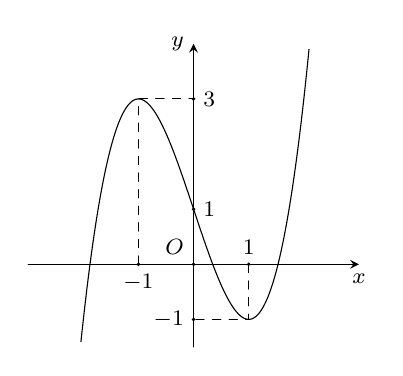
\begin{tikzpicture}[scale=0.7, font=\footnotesize, line join=round, line cap=round,>=stealth]
		\def\xmin{-3} \def\xmax{3}
		\def\ymin{-1.5} \def\ymax{4} 		
		\draw[->] (\xmin,0)--(\xmax,0) node [below]{$x$};
		\draw[->] (0,\ymin)--(0,\ymax) node [left]{$y$};
		\node at (0,0) [above left]{$O$};
		\clip (\xmin+0.1,\ymin+0.1) rectangle (\xmax-0.1,\ymax-0.1);
		\draw[smooth,samples=300] plot(\x,{(\x)^3-3*(\x)+1});		
		\fill (0,0) circle (1.0pt) (1,0) circle (1.0pt) (-1,0) circle (1.0pt) (0,3) circle (1.0pt) (0,1) circle (1.0pt)node[right]{$1$} (0,-1) circle (1.0pt);
		\draw[dashed] (-1,0)node[below]{$-1$}--(-1,3)--(0,3)node[right]{$3$} 
		(1,0)node[above]{$1$}--(1,-1)--(0,-1)node[left]{$-1$};
		\end{tikzpicture}
	}
	\loigiai{
		Dựa vào đồ thị ta có: Đồ thị hàm số có điểm cực tiểu là $(1;-1)$ và điểm cực đại là $(-1;3)$.}
\end{ex}
\begin{ex}%Câu 17.%[2D1Y2-2]
	\immini{
		Cho đồ thị hàm $y=f(x)$ như hình vẽ. Số điểm cực trị của đồ thị hàm số là	
	\choice
	{$4$}
	{$3$}
	{\True $5$}
	{$2$}
	}{
		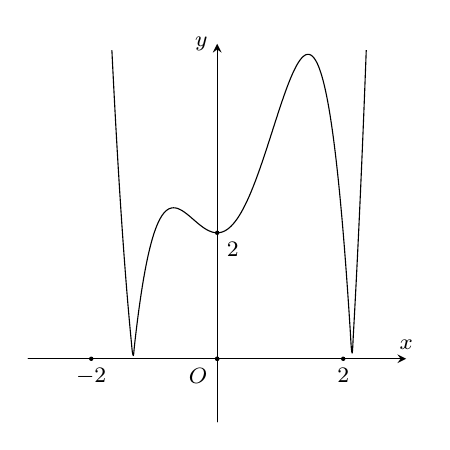
\begin{tikzpicture}[scale=0.8, font=\footnotesize, line join=round, line cap=round,>=stealth]
		\def\a{-1}  % Hệ số co dãn
		\def\xmin{-3} \def\xmax{3}
		\def\ymin{-1} \def\ymax{5} 		
		\draw[->] (\xmin,0)--(\xmax,0) node [above]{$x$};
		\draw[->] (0,\ymin)--(0,\ymax) node [left]{$y$};
		\node at (0,0) [below left]{$O$};
		\clip (\xmin+0.1,\ymin+0.1) rectangle (\xmax-0.1,\ymax-0.1);
		\draw[smooth,samples=300,domain=-2.5:2.5] plot(\x,{abs(\a*((\x+1)*(\x)^2*(\x-2))+2)});
		\fill (0,0) circle (1.0pt);
		\fill (0,0) circle (1.0pt) (2,0) circle (1.0pt)node[below]{$2$}  (-2,0) circle (1.0pt)node[below]{$-2$} (0,2) circle (1.0pt)node[below right]{$2$};
		\end{tikzpicture}
	}
	\loigiai{
		Đồ thị hàm số có 5 điểm cực trị.\\
		Chú ý, tại các điểm mà đồ thị có dạng “nhọn” thì đó vẫn là điểm cực trị của đồ thị hàm số.}
\end{ex}
\begin{ex}%Câu 18.%[2D1B2-1]
	Cho hàm số $y=f(x)$ có đúng ba điểm cực trị là $-2$; $-1$, $0$ và có đạo hàm liên tục trên $\mathbb{R}$. Khi đó hàm số $y=f\left(x^2-2x\right)$ có bao nhiêu điểm cực trị?
	\choice
	{\True $3$}
	{$8$}
	{$10$}
	{$7$}
	\loigiai{
		Vì hàm số $y=f(x)$ có đúng ba điểm cực trị là $-2$; $-1$, $0$ và có đạo hàm liên tục trên $\mathbb{R}$ nên $f'(x)=0$ có đúng ba nghiệm bội lẻ là $-2$; $-1$, $0$.\\
		Xét hàm số $y=f\left(x^2-2x\right)$ có $y'=(2x-2)\cdot f'\left(x^2-2x\right)$.\\
		$y'=0\Leftrightarrow(2x-2)\cdot f'\left(x^2-2x\right)=0\Rightarrow\hoac{&x=1\\&x^2-2x=-2\\&x^2-2x=-1\\&x^2-2x=0}\Leftrightarrow\hoac{&x=1\\&x=0\\&x=2.}$ \\
		Khi đó $y'=0$ có ba nghiệm bội lẻ $0$; $1$; $2$ nên hàm số $y=f\left(x^2-2x\right)$ chỉ có ba điểm cực trị.}
\end{ex}
\begin{ex}%Câu 19.%[2D1K2-2]
	\immini{
		Cho hàm số $y=f(x)$. Biết rằng hàm số $y=f'(x)$ liên tục trên $\mathbb{R}$ và có đồ thị như hình vẽ bên. Hỏi hàm số $y=f\left(5-x^2\right)$ có bao nhiêu điểm cực trị?	
	\choice
	{\True $7$}
	{$9$}
	{$4$}
	{$3$}
	}{
		\begin{tikzpicture}[scale=0.6, font=\footnotesize, line join=round, line cap=round,>=stealth]
		\def\a{1/9}  % Hệ số co dãn
		\def\xmin{-5} \def\xmax{5}
		\def\ymin{-2.5} \def\ymax{5} 		
		\draw[->] (\xmin,0)--(\xmax,0) node [above]{$x$};
		\draw[->] (0,\ymin)--(0,\ymax) node [left]{$y$};
		\node at (0,0) [above left]{$O$};
		\clip (\xmin+0.1,\ymin+0.1) rectangle (\xmax-0.1,\ymax-0.1);
		\draw[smooth,samples=300] plot(\x,{\a*((\x+4)*(\x-1)*(\x-4))});
		\fill (0,0) circle (1.0pt);
		\fill (0,0) circle (1.0pt) (1,0) circle (1.0pt)node[below]{$1$}  (-4,0) circle (1.0pt)node[above left]{$-4$} (4,0) circle (1.0pt)node[below right]{$4$};
		\end{tikzpicture}
	}
	\loigiai{
		Ta có $y'=-2xf'\left(5-x^2\right)\Leftrightarrow\hoac{&x=0\\&5-x^2=-4\\&5-x^2=1\\&5-x^2=4}\Leftrightarrow\hoac{&x=0\\&x=\pm 3\\&x=\pm 2\\&x=\pm 1.}$ \\
		Ta có BBT
		\begin{center}
			\begin{tikzpicture}
			\tkzTabInit[nocadre=false,lgt=1.2,espcl=2,deltacl=0.6]
			{$x$ /0.6,$-2x$/0.6,$y'$ /0.6, $y$ /2}
			{$-\infty$,$-3$,$-2$,$-1$,$0$,$1$,$2$,$3$,$+\infty$}
			\tkzTabLine{,+,|,+,|,+,|,+,$0$,-,|,-,|,-,|,-,}
			\tkzTabLine{,-,$0$,+,$0$,-,$0$,+,$0$,+,$0$,-,$0$,+,$0$,-,}
			\tkzTabVar{+/, -/,+/,-/,+/, -/,+/, -/,+/,}
			\end{tikzpicture}
		\end{center}		
		$\Rightarrow$ hàm số $y=f\left(5-x^2\right)$ có $7$ điểm cực trị.}
\end{ex}
\begin{ex}%Câu 20.%[2D1K2-2]
	\immini{
		Cho hàm số $y=f(x)$ có đạo hàm và liên tục trên $\mathbb{R}$, có đồ thị hàm $y=f'(x)$ như hình vẽ. Tìm số điểm cực trị của hàm số $y=f(x-2019)+2017x-2018$. 
	\choice
	{\True $1$}
	{$2$}
	{$3$}
	{$4$}
	}{
		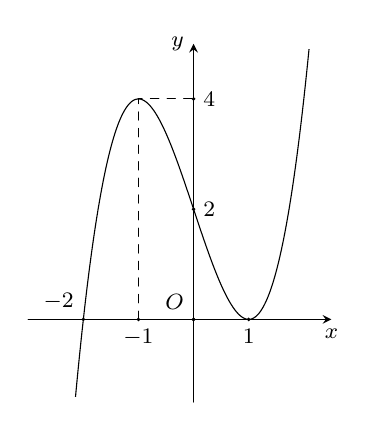
\begin{tikzpicture}[scale=0.7, font=\footnotesize, line join=round, line cap=round,>=stealth]
		\def\a{1}  % Hệ số co dãn
		\def\xmin{-3} \def\xmax{2.5}
		\def\ymin{-1.5} \def\ymax{5} 		
		\draw[->] (\xmin,0)--(\xmax,0) node [below]{$x$};
		\draw[->] (0,\ymin)--(0,\ymax) node [left]{$y$};
		\node at (0,0) [above left]{$O$};
		\clip (\xmin+0.1,\ymin+0.1) rectangle (\xmax-0.1,\ymax-0.1);
		\draw[smooth,samples=300] plot(\x,{\a*((\x+2)*(\x-1)*(\x-1))});
		\fill (0,0) circle (1.0pt);
		\fill (0,0) circle (1.0pt) (1,0) circle (1.0pt)node[below]{$1$} (-1,0) circle (1.0pt) (0,4) circle (1.0pt) (-2,0) circle (1.0pt)node[above left]{$-2$} (0,2) circle (1.0pt)node[right]{$2$};
		\draw[dashed] (-1,0)node[below]{$-1$}--(-1,4)--(0,4)node[right]{$4$};
		\end{tikzpicture}
	}
	\loigiai{
		Ta có $y=f(x-2019)+2017x-2018$ suy ra $y'=f'(x-2019)+2017$.\\
		Tịnh tiến đồ thị ta thấy $y'=f'(x-2019)+2017$ cắt trục $Ox$ tại $1$ điểm.\\
		Do đó hàm số có $1$ cực trị.}
\end{ex}
\Closesolutionfile{ans}